\chapter{はじめに}
\label{chp:first}

\section{背景} 
\label{sec:paragraph}
私が本研究に至った理由には私の二つの趣味が大きく関係している．その趣味の一つがパズルを解くことである．
似たものにクイズあるが，クイズが知識で答えを出すものであるのに対し，パズルは思考力で解くものであり，
そういった思考が私を非常に楽しくさせてくれるため，自身の趣味でありながらも自身の研究にしようと思った．

さて，単にパズルと言っても様々種類がある．クロスワードパズルのように答えを書き込みながら完成させていくペンシルパズル，
モンティーホール問題など論理的思考力を試すロジックパズル，
知恵の輪やルービックキューブで馴染みのある立体パズル，そしてジグソーパズルやスライディングブロックのような平面パズル．
他にも本当にたくさんのパズルがこの世の中には存在する．
では，これだけあるパズルの中でなぜ私がスライディングブロックパズルを本研究の題材に選んだか，それは私のもう一つの趣味が絵画鑑賞で自分の研究で絵画を扱いたいと思っていたからである．
自分の好きなパズルと絵画を組み合わせて何か出来ないかと考え，それを考慮すると平面パズルが都合が良く，その中でもスライディングブロックパズルを採用すれば，任意の二つの画像を
パズルの完成前・後の絵になるようにパズルを作ることができる上に，一枚の画像が違う画像に変化するアニメーションも得られるのではないかと私は思いついた．
しかしながら，凡人の私が考えていることなど他の誰かも当然考えており，先行研究\cite{makita}で既に同じような研究がなされていた．私が初めてだと思っていた分，少し悲しい気持ちになったが
その先行研究を読み進めているといくつか改善できる点が見つかり，自分ならもっとうまくできると思い，本研究に帰着した．

% しかしながら、例えば \verb+\verb+ 環境やインライン数式を用いる場合などで、
% \verb+abcdefghijklmnopqrstuvwxyzABCDEFGHIJKLMNOPQRSTUVWXYZ+ 
% というようにページ幅を超えてしまったり、前の行が間延びしてしまうようなケースがある。
% そのような場合、\verb+\\+ を用いて強制改行により \\
% \verb+abcdefghijklmnopqrstuvwxyzABCDEFGHIJKLMNOPQRSTUVWXYZ+ 
% というように用いるとよい。

\section{本論文の目的と構成}
\label{sec:enum}
私が本研究で用いるのは，スライディングブロックパズルの中でも代表的なパズルとされる15パズルである．
15パズルとは，\(4 \times 4\)のボード上に\(4 \times 4−1\)すなわち15枚の駒があり，1駒分の空きを利用して駒をスライドし，駒を目的の配置にするものである．本研究では15駒ではなく，これをさらに拡張し一辺の駒の数を$n$個とする合計で\(n^2-1\)個の駒を用いたパズルを採用した．
以降，これを\(n^2-1\)パズルと呼ぶ．

先行研究\cite{makita}では，まず正方形かつ大きさの同じ二つの画像と整数\(n\)を入力として与え，画像はグレースケール変換する．
そして，一つの画像を\(n \times n\)個の正方形に分割した\(n^2-1\)パズルとして並べ替えて再構築し，もう一つの画像に近似させる．
しかし，これでは元の画像に対して，再構築後の画像が近似された画像であるため，アニメーションにした時に変化前と後で絵の再現度にギャップが生じてしまう．
人間の感動というものは相対的なものであること(ヴェーバー・フェヒナーの法則)から，変化後の画像の再現度が高かったとしても変化前のオリジナルの画像には及ばないため，
このギャップがどうしても感動が薄くなる原因を作ってしまうのである．
そこで私はこの問題を，両方の画像の要素を含んだ新しい駒を作ることによって解決できるのではないかと考えた．
つまり，一方だけの再現度を落とすのではなく，両方とも同じように落とせば，前後でギャップもなくなり，変化後の再現度も先行研究よりも高くすることが可能になるということである．
以下が，その近似例\ref{fig:example1}である．
\begin{figure}[H]
  \centering
  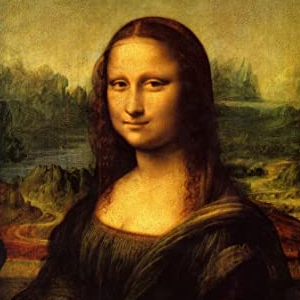
\includegraphics[width=3cm]{./fig/monariza.png}
  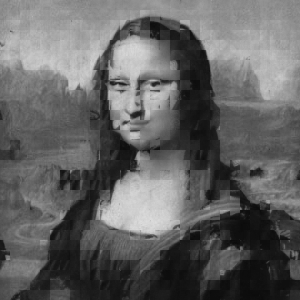
\includegraphics[width=3cm]{./fig/monariza2.png}
  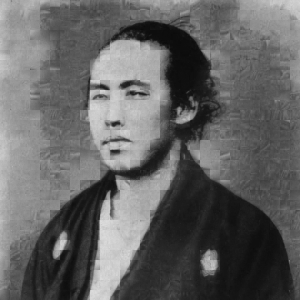
\includegraphics[width=3cm]{./fig/ryoma2.png}
  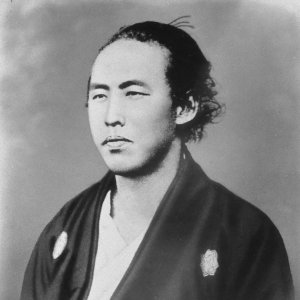
\includegraphics[width=3cm]{./fig/ryoma.png}
  \caption{近似例（30×30分割）}
% \url{http://www.this.is.sample.url/} % Web上のデータの場合、参照先URLを明記
  \label{fig:example1}
\end{figure}

また，\(n^2-1\)パズルの解き方についても手数面，芸術面において改善すべき点がいくつかあった．
以上2点を総合して改善することを本研究の目的とする．

本論文は，全5章から構成される．第1章では，背景と本論文の目的と構成について述べる．第2章では，スライディングブロックパズルの紹介や先行研究，そして本研究でのパズルの解法について述べる．
第3章では，本研究で提案する手法について述べる．第4章では，実験結果を画像と共に記載し，第5章では以上の結果より考察を述べる．
% \begin{enumerate}
%  \item 数字の付いた箇条書きの例
%  \item こんな感じで手順などを列挙
% \end{enumerate}

% 数字を付けずに列挙したい場合は itemize 環境を使う。
% このようにあるキーワードを指定して \verb+\begin(}+ と \verb+\end{}+ で
% 囲む範囲のことを○○環境と呼ぶ。

% \begin{itemize}
%  \item 順番などを伴わない箇条書きの例
%  \item 材料や要素を純粋に列挙したい場合に使用
% \end{itemize}

% enumerate 環境や itemize 環境は、入れ子構造を持つことができる。
% 例えば enumerate 環境の場合、以下のようになる。
% \begin{enumerate}
%  \item 東京都
%  \begin{enumerate}
%   \item 八王子市
%   \item 多摩市
%  \end{enumerate}
%  \item 神奈川県
%  \begin{enumerate}
%   \item 横浜市
%   \item 川崎市
%  \end{enumerate}
%  \item 山梨県
% \end{enumerate}

% \section{図表と参照}
% \label{sec:fig_tbl}

% 図を挿入する際は以下のように書く。
% 必ずキャプションを付けるとともに、図に対する説明を本文中で記載すること。
% 何かの手違いで図が表示されなくなったとしても、文章で意味が通じるくらいに説明するのを目安にすること。
% 以下の図 \ref{fig:sample} と図 \ref{fig:ferret} は、適当なサンプル画像である。

% \begin{figure}[H]
%   \centering
%   
\includegraphics[width=6.4cm]{./fig/fig-sample.eps}
%   \caption{適当なサンプル}
% % \url{http://www.this.is.sample.url/} % Web上のデータの場合、参照先URLを明記
%   \label{fig:sample}
% \end{figure}

% \begin{figure}[H]
%   \centering
%   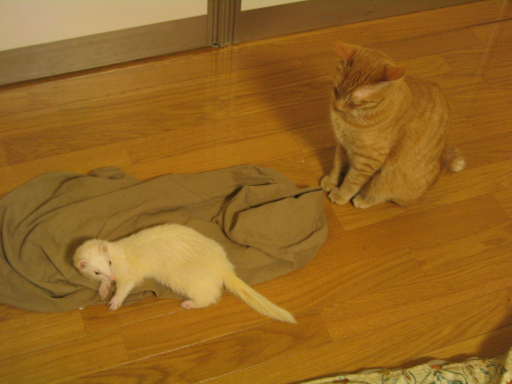
\includegraphics[width=6.4truecm]{./fig/ferret.png}
%   \caption{適当なサンプル2}
% % \url{http://www.this.is.sample.url/} % Web上のデータの場合、参照先URLを明記
%   \label{fig:ferret}
% \end{figure}

% これまで、\LaTeX での図は伝統的には EPS 形式が用いられてきたが、
% 近年では JPEG 形式や PNG 形式など多くの画像フォーマットに対応している。
% Inkscape や Illustrator 等のように直接 EPS 形式を出力する場合は EPS を用いることが望ましいが、
% それ以外の状況では EPS への変換は行わずに画像ファイルを直接指定した方が品質が良い。
% ただし、JPEG や PNG などの画像ファイルは EPS に比べて \LaTeX のコンパイルが長時間になる傾向があり、
% あまり巨大な画像データを使用するとかなりコンパイル時間が長くなってしまうので、注意が必要である。
% また、使用する画像ファイルはこのテンプレートのように
% fig サブフォルダ内に格納することを推奨する。

% 図への参照は \verb+\label+ コマンドを用いて各図のキャプションにキーワードを付けておき、
% 文中で \verb+\ref+ コマンドによってキーワードを指定することで記述する。
% キーワードは参照対象に応じてプリフィクスを付けることが望ましい。
% 以下の表 \ref{tbl:pre_list} に一般的に用いる参照対象ごとのプリフィクスを挙げる。

% \begin{table}[H]
%   \caption{ラベルに指定するキーワードのプリフィクス一覧}
%   \label{tbl:pre_list}
%   \centering
%   \begin{tabular}{|l|l|r|} \hline
%    参照対象	& プリフィクス \\ \hline
%    章		& chp: \\ \hline
%    節		& sec: \\ \hline
%    図		& fig: \\ \hline
%    表 		& tbl: \\ \hline
%    式   	& eqn: \\ \hline
%   \end{tabular}
% \end{table}
% 手作業でのナンバリングは非効率極まりない上に必ずミスが出るので行わないこと。

% \section{\LaTeX のコンパイル}
% \LaTeX のコンパイルは、「コマンドプロンプト」や「PowerShell」などのコマンドライン上で「
% latexmk」コマンドを用いる。
% 例えば、「M01xxyyy.tex」というファイルから PDF を作成したい場合は
% \begin{verbatim}
%     latexmk M01xxyyy
% \end{verbatim}
% というように、拡張子を抜いてコマンドラインで指定する。

% また、コマンドラインに不慣れな学生は、
% Atom エディタ等の \LaTeX パッケージを用いることも良案である。
% Atom エディタを用いた \LaTeX の記述については、研究室 Wiki を参照のこと。
